\documentclass[a4paper,12pt]{article}
\usepackage{amsmath}
\usepackage{amssymb}
\usepackage[polish]{babel}
\usepackage{polski}
\usepackage[utf8]{inputenc}
\usepackage{indentfirst}
\usepackage{geometry}
\usepackage{array}
\usepackage[pdftex]{color,graphicx}
\usepackage{subfigure}
\usepackage{afterpage}
\usepackage{setspace}
\usepackage{color}
\usepackage{wrapfig}
\usepackage{listings}
\usepackage{datetime}
\usepackage[outdir=./]{epstopdf}

\renewcommand{\onehalfspacing}{\setstretch{1.6}}

\geometry{tmargin=2.5cm,bmargin=2.5cm,lmargin=2.5cm,rmargin=2.5cm}
\setlength{\parindent}{1cm}
\setlength{\parskip}{0mm}

\newenvironment{lista}{
\begin{itemize}
  \setlength{\itemsep}{1pt}
  \setlength{\parskip}{0pt}
  \setlength{\parsep}{0pt}
}{\end{itemize}}

\newcommand{\linia}{\rule{\linewidth}{0.4mm}}

\definecolor{lbcolor}{rgb}{0.95,0.95,0.95}
\lstset{
    backgroundcolor=\color{lbcolor},
    tabsize=4,
  language=C++,
  captionpos=b,
  tabsize=3,
  frame=lines,
  numbers=left,
  numberstyle=\tiny,
  numbersep=5pt,
  breaklines=true,
  showstringspaces=false,
  basicstyle=\footnotesize,
  identifierstyle=\color{magenta},
  keywordstyle=\color[rgb]{0,0,1},
  stringstyle=\color{red}
  }

\begin{document}

\noindent
\begin{tabular}{|c|p{11cm}|c|} \hline 
Grupa 1 & Kordian Kurdziel, Mateusz Maciejak & \ddmmyyyydate\today \tabularnewline
\hline 
\end{tabular}


\section*{Zadanie 2 - Rozmycie Gaussa w MPI}

Zadaniem programu było rozmycie obrazu podanego na wejściu za pomocą algorytmu Gaussa z maską 5x5. W celu poprawy wydajności programu do zrównoleglenia jego działania należało wykorzystać standard MPI.
Program przyjmuje dwa argumenty, obraz wejściowy oraz obraz wyjściowy. Liczbę procesów na jakich mają zostać wykoanane obliczenia należy podać po komendzie mpirun używając flagi -n.

Do obsługi operacji na zdjęciu została wykorzystana biblioteka OpenCV. Poniższy fragment kodu prezentuje inicjalizację programu opartego o MPI oraz pobranie identyfikatora aktualnego procesu oraz liczby procesów z jaką został uruchomiony program. Jest to potrzebne do zrównloleglenia obliczeń w dalszej części programu.

\begin{lstlisting}
    MPI_Init(&argc, &argv);
    MPI_Comm_rank (commmunicate, &rank);
    MPI_Comm_size(commmunicate, &numberOfProcesses);
\end{lstlisting}

Funkcja MPI\_Init inicjuje mechanizm MPI. Następnie funkcja MPI\_Comm\_rank inicjuje do zmiennej rank aktualnie używany id procesu. Funkcja MPI\_Comm\_size ustawia w zmiennej numberOfProcesses ilość procesów.
Obrazek jest dzielony na równe części i rozdzielany przez proces główny na do oddzielnych procesów, które w separacji rozmywają kolejne partie obrazu. Do pocięcia obrazka wykorzystywana jest funkcja biblioteki OpenCv Rect.

\begin{lstlisting}
  cv::Rect myROI(x, y, width, height);
	cv::Mat croppedRef(picture, myROI);
	cv::Mat cropped;
\end{lstlisting}

Do komunikacji między procesami wykorzystane zostały funkcje standardu MPI - MPI\_Send i MPI\_Recv. Na poniższym listingu można zobaczyć ich sygnaturę.

\begin{lstlisting}
  MPI_Send(
      void* data,
      int count,
      MPI_Datatype datatype,
      int destination,
      int tag,
      MPI_Comm communicator)
  MPI_Recv(
      void* data,
      int count,
      MPI_Datatype datatype,
      int source,
      int tag,
      MPI_Comm communicator,
      MPI_Status* status)
\end{lstlisting}

W programie główny proces służy do odczytu obrazka, podzieleniu go na równe partie, wysłaniu do procesów podrzędnych i po przetworzeniu złączenie z powrotem do spójnej całości.
Główny jak i pozostałe procesy mogą być rozpoznane dzięki identyfikatorowi zwracanemu przez funckję MPI\_Com\_rank na początku programu. Poniższy fragment kodu przedstawia podzielenie obrazka na częśi i przesłanie ich do podrzędnych procesów.

\begin{lstlisting}
        // Split picture and send to other processes
        for (int i = 1; i < numberOfProcesses; ++i){

            partOfImg = cutPicture(inputImg, 0, (i -1) * imgSplitSize, inputImg.cols, imgSplitSize);

            x = partOfImg.rows;
            y = partOfImg.cols;
            
            send(&x, 1, MPI_INT, i, START_VALUE_TAG);
            send(&y, 1, MPI_INT, i, END_VALUE_TAG);
            send(partOfImg.data, x * y * 3, MPI_BYTE, i, DATA_TAG);
        }
\end{lstlisting}

Samo rozmycie obrazu jest analogiczne jak w zadaniu numer 1.

Poniższe wykresy 1 i 2, przedstawiające zależność czasową oraz przyspieszenia zostały oparte na średnich wynikach programu uruchamianych lokalnie na maszynie wirtualnej. Wykorzystany został 6 rdzeniowy procesor Intel z technologią Hyperthreadingu.

\begin{figure}[!ht]
	\centering
  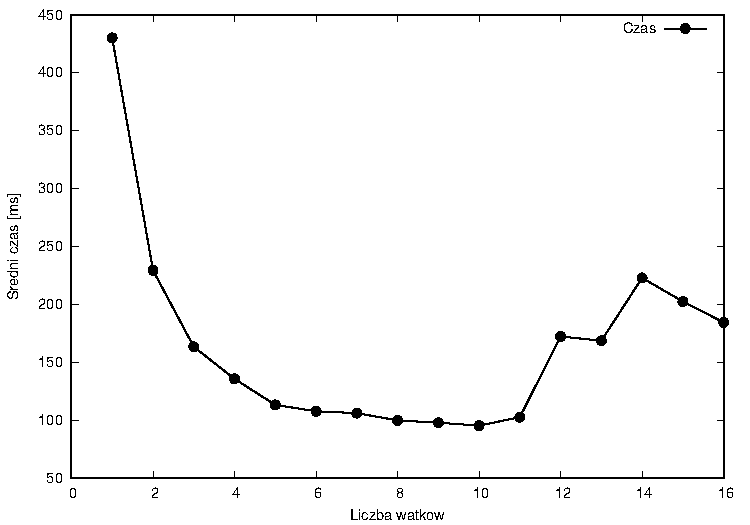
\includegraphics[width=0.5\textwidth]{wykresCzas.pdf}
  \caption{Wykres zależności czasu wykonywania obliczeń od liczby wątków}
\end{figure}

\begin{figure}[!ht]
	\centering
  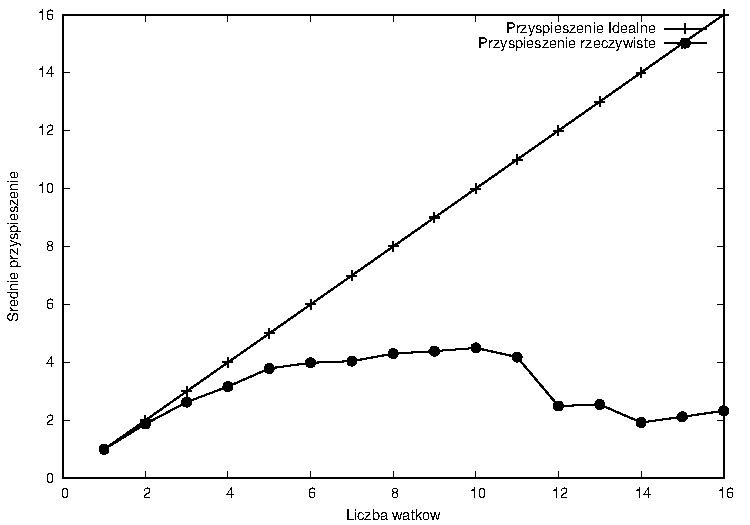
\includegraphics[width=0.5\textwidth]{wykresPrzyspieszenie.pdf}
  \caption{Wykres przyspieszenia działania programu w zależności od liczby wątków}
\end{figure}
Można zauważyć, że po przekroczeniu fizycznej liczby rdzeni wydajność przestaje rosnąć, a więc HyperThreading nie dodaje zauważalnej różnicy w tym zadaniu. Po dalszym zwiększaniu liczby wątków wydajność programu zaczyna drastycznie maleć, co świadczy o dużych nakładach związanych z tworzeniem i komunikacją międzywątkową.



\end{document}
